\chapter{Introduction}
\label{chap:intro}

Online Educational Systems is an emerging technology nowadays. It started with school level education for courses like Maths, English, etc. Presently, online courses are available for many technical and advanced studies. 

Earlier, classroom teaching was the only way to impart education. It has been an effective mode of education for several ages, but it has constraints. There are always students in a class who are not able to interact much with their professors or classmates. Classroom education is restricted to a particular physical location, so it is not available to a significantly large audience. Above that, classrooms are generally conducted for a limited time and hence it is not possible to solve all the queries or doubts of students, then and there.

Now, an alternative method is evolving to solve the problems of classroom education. Online Educational Systems are generally interactive in nature. Students can be provided with questions for practice which can be evaluated by the system itself. This reduces the overhead of instructor and hence allows accomodation of a large number of students in the course. Problems can also be generated by such systems. Some systems also provide feedback to the students after evaluating their answers.

In this thesis, we propose an Online Educational System for Compilers. This has been created for the parsing phase of Compilers. The results of which have been detailed in Chapter. %_________.

\section{Objective}
\label{objective}
The purpose of this Thesis is to create an Online Tutoring System for Compilers. The main objective is to generate problems automatically and evaluate the solution to those problems, which are submitted by the students. If a solution is wrong, then the system generates hint problems which guide the student to reach to the correct solution to the main problem. Otherwise it generates the next main problem. This work-flow is accomplished by calculating the solution to the problem beforehand. This pre-computed solution is then compared with the solution given by the student. The goal of this thesis is to generate problems automatically and provide immediate feedback to the students, while solving problems. 

\section{Motivation of Work}
\label{motivation}
Students generally face a lot of problems in learning compiler technology. They do not understand the different techniques involved in various phases of program compilation. Parsing is one of such phases, which consists of a large number of techniques. Students face many problems in grasping these techniques.

Parsing techniques mostly follow different algorithms to solve a parsing problem. This requires a step by step method to reach to the solution to such a problem. If a student makes a mistake in even one step, then the result is completely wrong. It is also very difficult for the student or the instructor to figure out such a mistake as it involves recalculation of all the steps.

Therefore, we needed a system that can provide students with a large number of problems for practice. We also needed to make them realise their mistakes by generating feedback. Feedback is a necessary step to guide a student to the correct solution. Our feedback provide students with hint questions of different types to make them understand what went wrong and how to reach to the correct solution.

\section{Outline of the Solution}
\label{outline}
The system is divided into three parts. Figure 1.1 gives an abstract view of the system.
\begin{figure}[h]
\centering
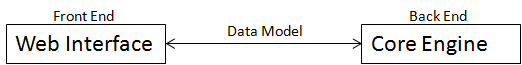
\includegraphics{Figure1.png}
\caption{Framework of the System}
\label{fig:framework}
\end{figure}

The system is mainly consists of:
\begin{itemize}
\item \textbf{Core Engine:} This part of the system deals with generation of problems, evaluation the answers given by students and generating hint questions automatically based on the answer given by students.
\item \textbf{Data Model:} It acts as an interface between front-end and back-end. It is used to transfer data back-and-forth between core engine and web interface.
\item \textbf{Web Interface:} This part provides a user-friendly environment to the student. It deals with the presentation of problems and provides ease of giving solutions.
\end{itemize}

\section{Contribution of Thesis}
\label{contribution}
In this thesis, we have implemented a tool for the parsing phase of program compilation. It generates problems automatically for the different techniques involved in this phase, i.e. First set, Follow set, LL Parsing (which includes LL Parsing Table and LL Parsing Moves) and SLR Parsing (which includes SLR Canonical set, SLR Parsing Table and SLR Parsing Moves). We have tested the system on various grammars. The system also includes functionality like generation of input strings for a particular cell of the LL Parsing Table (in which a student has made a wrong entry while filling the table) and showing LL Parsing moves on that string to make the student understand, why the value she entered in the cell is incorrect.

\section{Thesis Organization}
\label{organization}
Rest of the thesis is organised as follows:

\textbf{Chapter 2},

\textbf{Chapter 3},

\textbf{Chapter 4},

\textbf{Chapter 5},

\textbf{Chapter 6},